%mention need for compression
\subsubsection{Tensor Network Diagrams}
\begin{figure}
  \centering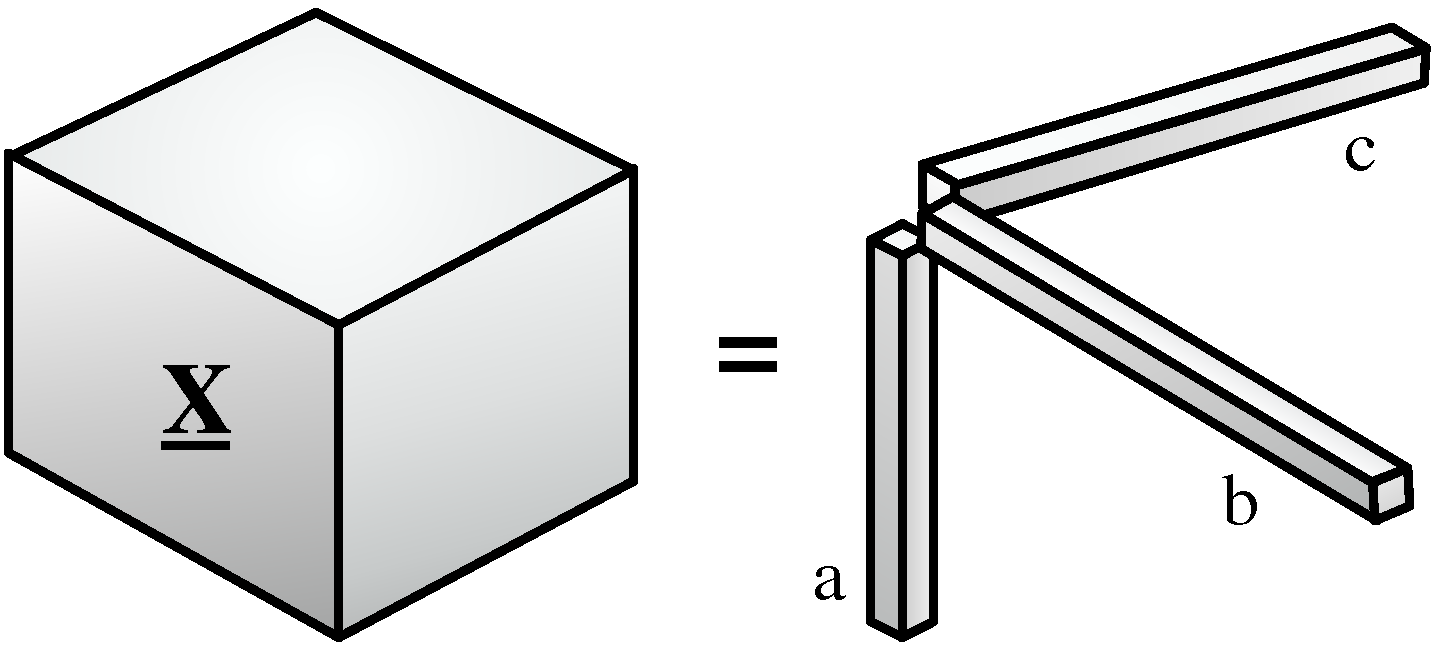
\includegraphics[width=0.5\linewidth]{figs/cpdecomp}
  \caption{CP Decomposition.}
  \label{fig:cpdecomp}
\end{figure}

\subsubsection{Tensor Network Diagrams}
\begin{figure}
  \centering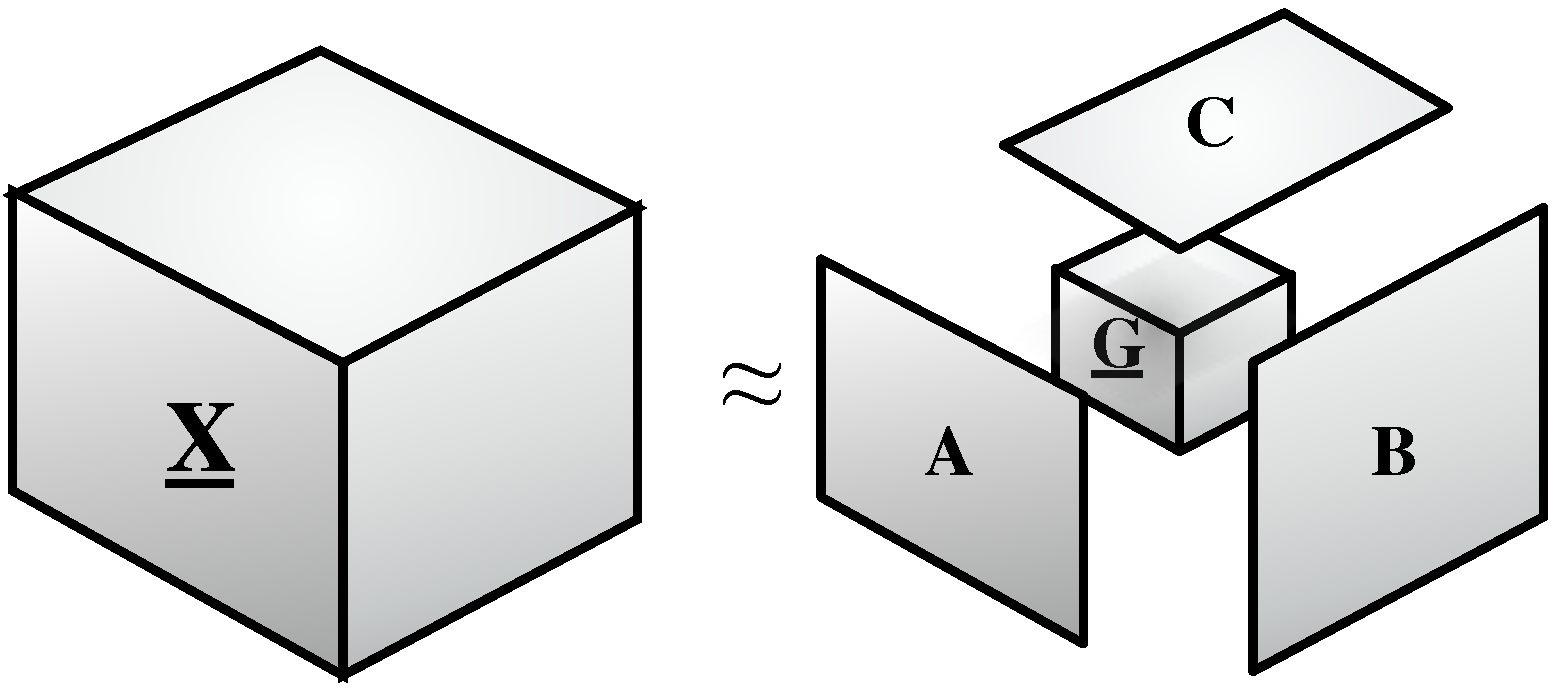
\includegraphics[width=0.55\linewidth]{figs/tdecomp}
  \caption{Tucker decomposition.}
  \label{fig:tdecomp}
\end{figure}

Tucker, CP are old concepts. Decomposition into block terms~\cite{Lathauwer08decompositionsof} generalizes standard methods.

Neat application: Bilinear maps can be generalized as tensors, so tensor decompositions can yield faster algorithms for matrix multiplication, i.e~\cite{Benson}

\subsection{CP Decomposition}
Introduced:~\cite{hitchcock-sum-1927}
CP breaks curse of dimensionality: instead of $n^d$ parameters we need only $dnr$.
CP is ill-posed, different regularizations can be used.
CP assumes every tensor mode is involved with every `concept.' Restrictive for noisy higher order data (-Joachim)
\subsection{Tucker Decomposition}
Introduced:~\cite{Tuck1966c}
Instead of $n^d$ parameters we need only $\prod_{i=1}^d r_i + n\sum_{i=1}^d r_i$.
Stable, we can use SVD~\cite{Lathauwer00amultilinear} To compute using `Tucker HOOI' algorithm~\cite{Lathauwer-THOOI}.
We can determine $r_1, \dots, r_d$ as a function of $\epsilon$.

If the Tucker Decomposition is properly normalized, it is also considered an HOSVD.

Exponential storage, time. In sparse case, we have same problem: dense results (-Joachim)
\subsection{Hierarchical Tucker}
Introduced:~\cite{Grasedyck:2010:HSV:1958286.1958311}
B's can express a linear combination of vectors in the U's below them.
Obst 1: SVD of tensor unfoldings
Obst 2: Intermediate memory blowup (computing core tensor)... dense intermediate result

Tree-adaptive algorithm using clustering~\cite{treeadap}

\subsubsection{Sparse H-Tucker}
If we use CUR decomposition instead of SVD and store only those columns and rows that contain an element, we can greatly reduce storage and retain sparsity of 

\subsection{Tensor Train}
Introduced:~\cite{Oseledets:2011:TD:2079141.2079149}
%=======================================================================

%eof
